\documentclass[11pt]{iopart}
%Uncomment next line if AMS fonts required
%\usepackage{iopams}
\usepackage{fancyhdr}
\usepackage{graphicx}
\usepackage{todonotes}
\usepackage{subfig}
\usepackage{ulem}

\usepackage[hidelinks]{hyperref}
\hypersetup{colorlinks=false}

\pagestyle{fancy}
\lhead{Diffusion Limited Aggregation}
\rhead{Candidate Number: 21594}

\begin{document}

%Makes TODO notes format properly in margin
\setlength{\marginparwidth}{1.5cm}

\title[]{The Effects of Simulation Parameters When Modelling Systems Using Diffusion Limited Aggregation}

\author{Candidate Number: 21594}

\address{Department of Physics,
University of Bath, Bath BA2 7AY, United Kingdom}
\begin{abstract}
Abstract goes here
\end{abstract}

\listoftodos

%Uncomment for PACS numbers title message
%\pacs{00.00, 20.00, 42.10}
% Keywords required only for MST, PB, PMB, PM, JOA, JOB? 
%\vspace{2pc}
%\noindent{\it Keywords}: Article preparation, IOP journals
% Uncomment for Submitted to journal title message
%\submitto{\JPA}
% Comment out if separate title page not required
%\maketitle


\section*{Preface}
Although the coursework was initially presented as a C++ project, I took the liberty of rewriting the DLA system in a programming language called Google Go. The motivation for this is Go more easily supports high concurrency. This means that instead of simulating 1 cluster at a time, 100 different clusters can be simulated simultaneously in different threads. To support this high level of concurrency, the results were generated by running the code on a 32-core virtual server. The code can be obtained by visiting https://github.com/hcoplestone/DLA.

\section{Introduction and Simulation Method}

Diffusion Limited Aggregation (DLA) is a theory that models the process of how clusters of particles grow, where growth is driven primarily by diffusion. \cite{dla}

\begin{figure}[h]
  \centering
  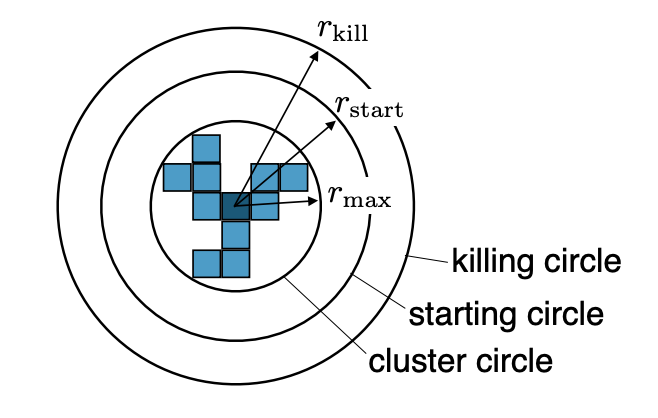
\includegraphics[width=0.5\linewidth]{images/circles.png}
  \caption{"Diagram of the circles used in the DLA code. The initial particle is shown in dark blue, and all circles are centred on this particle. There are three circles which indicate the approximate cluster size ('cluster circle'), the locations at which particles are introduced to the system ('starting circle'), and the points at which particles are removed from the system, to prevent them from wandering too far from the cluster ('killing circle')." Diagram and caption lifted verbatim from \cite{handout}.}
  \label{fig:circles}
\end{figure}

In the DLA method used in this paper, a stationary seed particle is placed at the centre of a square lattice. This defines the origin of our system, as shown in Figure 1. A particle is then added to the system at a radius $r_{start}$ from the origin. This radius is computed such that each new particle is added at a radius greater than any stationary particle in the system. Diffusion limited transport is driven by Brownian motion, a random process, so the new particle is made to undergo a random walk through the system. If the particle moves to a cell on the lattice that is horizontally or vertically adjacent to a stationary particle, the particle is stuck to the grid cell with a sticking probability $p_{stick}$. If the particle moves too far away from the cluster, as defined by a radius $r_{kill}$, the particle is removed from the system. Once a particle is stuck to the cluster or killed for walking too far away, a new particle is added and the process is repeated. The process is terminated when the cluster approaches the edge of the lattice or when a total number of particles in the cluster is achieved.

In this paper, we investigate whether the maximum number of particles used in a DLA system affects the fractal index of the generated cluster. We also investigate how fractal dimension depends on the sticking probability $d_f$, and link this to the thermodynamics of a growing system.

\section{Method}
\subsection{Random Walks and Ensemble Averaging}
To simulate the Brownian motion of diffusing particles, DLA simulations have free particles undergo a random walk. At each iteration, a number between 0 and 3 is 'randomly' generated, with each value representing a direction the particle can move in: up, right, down and left. The issue with this is that the sequence of random numbers generated is only 'pseudo-random'. For a given random number generator seed, the same sequence of numbers will always be generated. To mitigate this, an ensemble of systems are simulated, each with a different random number generator seed. For a given measurement $\xi(t)$, an ensemble average $\overline{\xi(t)}$ is calculated by averaging over $n$ independent systems $\{i\}_1^n$, where $i$ represents a specific simulated system:

\begin{equation}
\overline{\xi(t)} = \frac{1}{n}\sum_{i=1}^{n}{\xi_i(t)}
\end{equation}

Standard error can be used to estimate how close the ensemble average is to the true value:

\begin{equation}
\sigma_{\overline{\xi}} = \frac{1}{\sqrt{n-1}} \left[ \overline{\xi(t)^2} - \overline{\xi(t)}^2 \right]^{1/2}
\end{equation}

\subsection{Determining the Fractal Dimension of DLA Aggregates}

Talk about method of curve fitting. Talk about number of ensembles used. 

\subsection{Sticking Probabilities}

Talk about method of varying sticking probability and calculating sticking probability. Include values for number of particles, and number of ensembles.

\section{Results}
bla

\section{Discussion}
bla

\section{Conclusion}
bla

\section*{References}
\bibliography{refs}
\bibliographystyle{plain}

\end{document}

